%!TEX root = report.tex

\chapter{État de l'art}
\section{Introduction}
Dans ce chapitre on présente une étude de marché en énumérant
les applications dont les fonctionnalités sont équivalentes à la
notre tout en soulignent les différences qui subsistent. Ensuite on
présente la plate-forme \android{} et en passe en revu l'architecture
d'une application android.

\section{Étude de marché}
Plusieurs sociétés offre des solution en relation avec celle proposé
par ce présent rapport. Malheureusement, la plus par d'entre elle sont
des solutions commerciales et, faute de documentation disponible, on
n'a pas pu les étudier d'une point de vu techno-technique et on c'est
contenté de relayé leurs caractéristiques tel que présenté dans
les sources cités.

\paragraph{NB:} % (fold) 
\label{par:nb}

Les solutions présenté ici sont le fruit des sociétés bien établis avec des
ressources considérable et des salariés professionnels. Les comparé avec le
travail incubé dans ce rapport serai abusive, l'indulgence est de mise.

% paragraph nb (end)

\subsection{MIAA - Palomar Pomerado Health}

\begin{figure}
\centering
\subfloat{
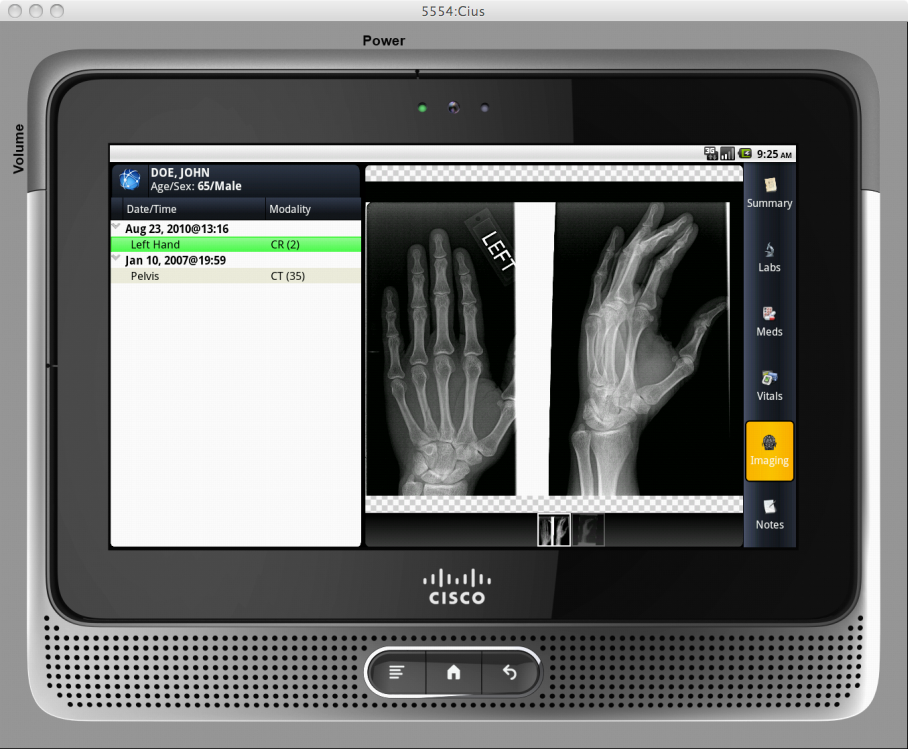
\includegraphics[width=0.5\textwidth]{pph1}
}\\
\subfloat{
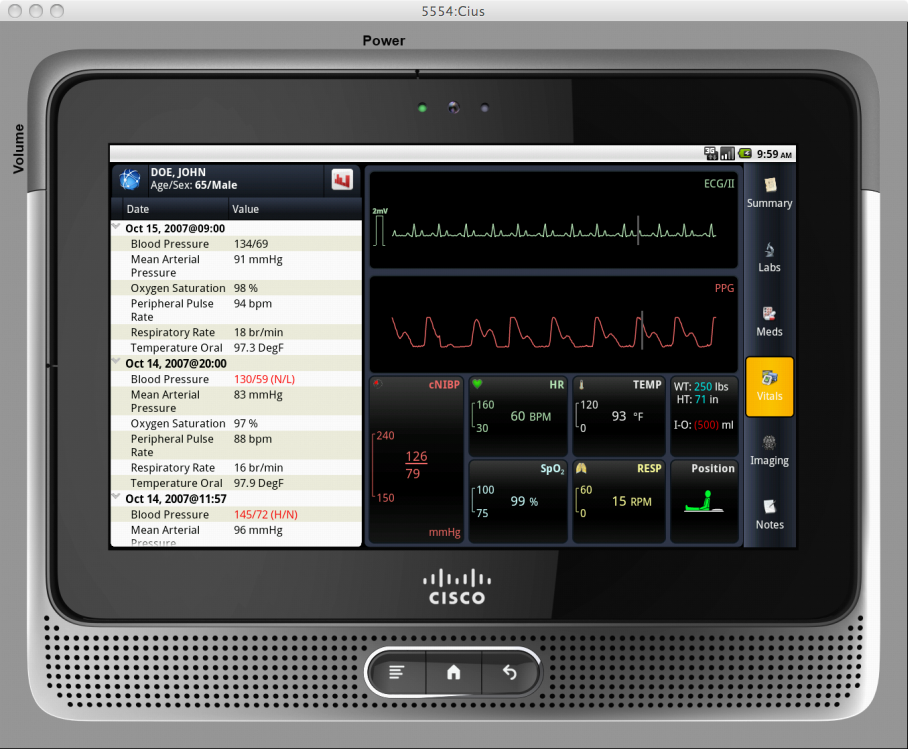
\includegraphics[width=0.5\textwidth]{pph2}
}\\
\subfloat{
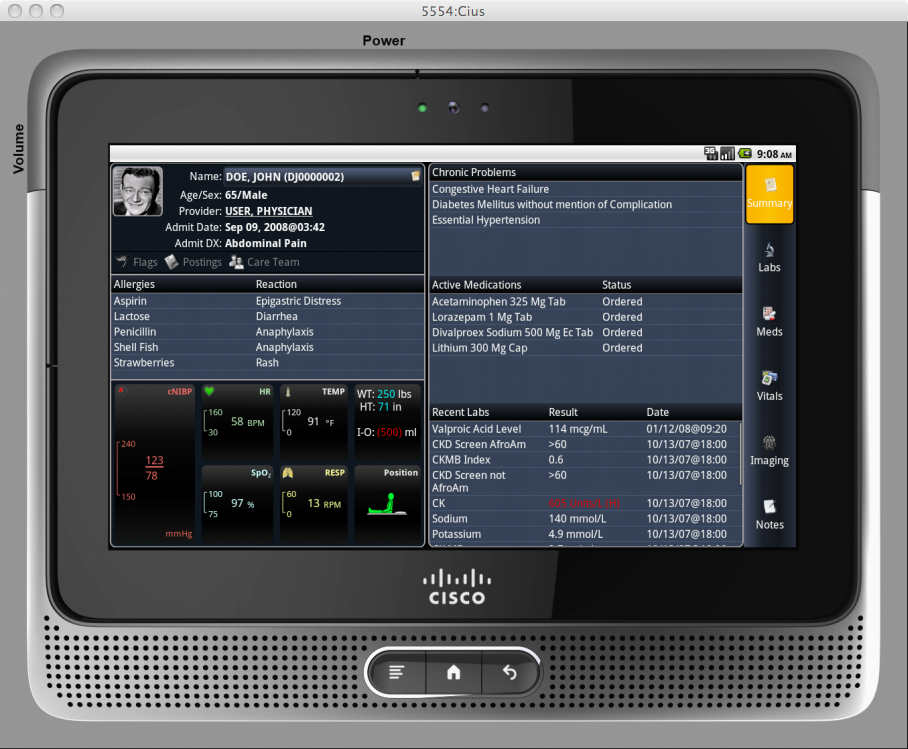
\includegraphics[width=0.5\textwidth]{pph3}
}
\caption{\gls{miaa} sur un émulateur Cisco Cius}
\label{fig:miaa}
\end{figure}

\gls{miaa} (figure \ref{fig:miaa}) est une application mobile issu d'un
projet R\&D chez \en{Palomar Pomerado Health}, l'institution public la
plus large dans l'état de Californie (USA). Elle permet au médecins
d'accédé rapidement au dossier médical complet du patient depuis une
variété de source différentes qui s\'affranchie des frontières des
organisation\cite{pph:eweek}. Elle vise les terminales équiper avec
le systéme d'exploitation \android{} comme les smartphones et les
tablettes. \en{Palomar Pomerado Health} a choisie de déployer cette
application dans le \en{Palomar Medical Center} à \en{Escondido}
(319 lits) et le \en{Pomerado Hospital} à \en{Poway} (107 lits) sur
des tablette Cisco Cius\cite{pph:tabtimes}, ce choix s'est basé sur le
support qu'offre Cisco pour ces divers équipements.
Les avantages de \gls{miaa} sont:~\cite{pph:yahoo}
\begin{itemize}
\item Application mobile facile à utilisé conçu spécifiquement aux
médecins, tournant sur la plate-forme \android{}.
\item Un service \en{Cloud} qui fournit un accès permanent à
l'historique médicale des patients à partir de divers sources de
données qui s\'affranchie des frontières des organisations.
\item Interopérabilité avec les pionniers des systèmes électroniques
de l'historique médicales tel que Cerner - \tm{Millennnium},
\tm{NextGen}, et \en{Veterans Administration} - \tm{VistA}.
\item Intégration en temps-réel des technologies de surveillance
des signes vitaux sans fils comme l'ECG, SPO$_{2}$, rythme cardiaque,
température, respiration, et pression du sang à partir des équipements
sans-fils.
\item Affichage des information génétique personnel.
\item Application dynamique qui s'ajuste automatiquement à l\'hôpital,
clinique, au à la maison.
\item Simple, facile à utilisé, avec une \gls{ui} tactile
de nouvelle génération.
\item Intégration d'une messagerie inter-médecins sécurisé tout en
maintenant le contexte du patient.
\item Des plan future pour intégré NHIN \en{Connect} et les services
\en{Direct}.
\end{itemize}

\subsection{\pct{} - Cerner}

\begin{figure}[H]
\centering

\includegraphics[width=0.3\textwidth]{logo_cerner}
\end{figure}

\pct{} est une solution mobile conçu par le laboratoire Cerner qui
fait parti de l'ensemble de solutions \tm{Millennium+} et qui permet de
facilité le travail des médecins. Elle offre une expérience native
sur iPad pour géré les visites médicales et permet aux médecins
d'effectuer tout une visite typique qui inclue:~\cite{pct:flyer}
\begin{itemize}
\item Consultation des emplois du temps et les chartes des patients.
\item Satisfaire les demandes récurrentes comme les commandes simple
et les recharges des médicaments.
\item Consultation des diagnostiques et résultats cliniques.
\item Documenté les allergies, les problèmes de santé et l'historique
du patient.
\item Crée et signé les notes de progressions.
\end{itemize}

Dé la fin du flux de travail du médecin ambulant. Cerner étend ces
même fonctions et les adaptes aux établissements hospitalier, les
urgences et les divers spécialistes.
Les avantages clés du \pct{} sont:~\cite{pct:flyer}
\begin{itemize}
\item Des réponses instantanés avec un flux de travail aisée.
\item Pas besoin de configuré l'application.
\item Adapter pour les visite médicales, aux patients et aux conditions
de la consultation.
\item Transmission sécurisé des données.
\item Des capacités de reconnaissance vocale.
\end{itemize}

\section{Le système d'exploitation \android{}}

\begin{figure}[H]
\begin{center}

\includegraphics[width=0.2\textwidth]{Android_robot.pdf}\\

\includegraphics[width=0.2\textwidth]{Android.pdf}
\end{center}
\caption{Logo et sigle d'\android{}}
\end{figure}

\android{} est un système d'exploitation basé sur \en{Linux} conçu pour les
équipements mobile avec d'un écran tactile comme les \en{smartphones} et les
tablettes. Développer à l'origine par \en{\android{}, Inc.} que \en{Google} a
supporté financièrement et plus-tard acquérir en 2005. \android{} a été
dévoilé en 2007 parallèlement a la fondation de l'\en{Open Handset Alliance}:
un consortium composé de sociétés dévoué a l'avancement des standards ouverts
pour les équipements mobile. Le première téléphone sous \android{} est vendu
en Octobre 2008.

La dernière version stable d'\android{} en date (Mai 2013) est 4.2.2 \en{
Jelly Bean} sortie le 11 Février 2013.

\android{} est basé sur le Kernel Linux et utilise pleinement ses capacités de support matériels exhaustif. Mais la comparaison avec les distribution Linux, embarqué ou même destiné aux bureaux, s'arrête a ce niveaux.~\cite{lft:growth_android}

\begin{figure}
\centering
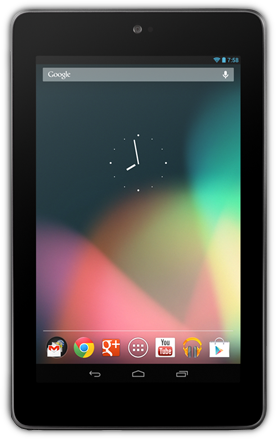
\includegraphics[width=0.4\textwidth]{nexus7}
\caption{\en{Google} Nexus 7, un terminal \android}
\end{figure}

\subsection{Parts du marché}
L’adoption du système d'exploitation \android suit une courbe exponentiel depuis quelque temps et la tendance n'est pas prête de s’inverser, selon les dernière rapport du cabiné d'analyse \en{Strategy Analytics}, \android a réussi à capturé environ 68.4\% du marché globale \cite{venturebeat.com}.

\begin{table}[H]
\centering
\begin{tabular}{|m{0.2\textwidth}|m{0.13\textwidth}|m{0.13\textwidth}|m{0.13\textwidth}|m{0.13\textwidth}|m{0.13\textwidth}|}
\hline
\textsf{Système d'exploitation} &
\textsf{Volume de production 3Q2012\footnotemark[1]\footnotemark[3]} &
\textsf{Parts du Marché 3Q2012\footnotemark[1]} &
\textsf{Volume de production 3Q2011\footnotemark[2]\footnotemark[3]} &
\textsf{Parts du Marché 3Q2011\footnotemark[2]} & \textsf{Différence} \\ 
\hline
\android{} & 136.0 & 75.0\% & 71.0 & 57.5\% & 91.5\% \\
\hline
iOS & 26.9 & 14.9\% & 17.1 & 13.8\% & 57.3\% \\
\hline
BlackBerry & 7.7 & 4.3\% & 11.8 & 9.5\% & -34.7\% \\
\hline
Symbian & 4.1 & 2.3\% & 18.1 & 14.6\%  & -77.3\% \\
\hline
Windows Phone 7/ Windows Mobile & 3.6 & 2.0\% & 1.5 & 1.2\% & 140.0\% \\
\hline
Linux & 2.8 & 1.5\% & 4.1 & 3.3\% & -31.7\% \\
\hline
Autres & 0.0 & 0.0\% & 0.1 & 0.1\% & -100.0\% \\
\hline
\hline
Totales & 181.1 & 100.0\% & 123.7 & 100.0\% & 46.4\% \\ \hline
\end{tabular}
\caption{Les six major systèmes d'exploitation mobile en terme de Volume
et du parts de marché en 3\ieme trimestre 2012~\cite{idc}}
\label{tab:marketshareall}
\end{table}

\footnotetext[1]{3\ieme trimestre 2012}
\footnotetext[2]{3\ieme trimestre 2011}
\footnotetext[3]{En million d'unité}

\begin{table}[H]
\centering
\begin{tabular}{|m{0.3\textwidth}|m{0.1\textwidth}|m{0.1\textwidth}|m{0.1\textwidth}|m{0.1\textwidth}|m{0.1\textwidth}|}
\hline
& \textsf{2008} & \textsf{2009} & \textsf{2010} & \textsf{2011} &
\textsf{2012}\footnotemark[4]\\
\hline
\textsf{Unités \android{} produites} & 0.7 & 7.0 & 71.1 & 243.4 & 333.6\\
\hline
\textsf{Parts de marché \android{}} & 0.5\% & 4.0\% & 23.3\% & 49.2\%
& 68.2\%\\
\hline
\end{tabular}
\caption{Production et parts de marché entre 2008 et 2012~\cite{idc}}
\label{tab:marketshare}
\end{table}

\footnotetext[4]{Estimation}

\subsection{Versions \android{} en circulation}
Le tableaux \ref{tab:androidversion} représente les différentes versions
d'\android{} et leurs taux d'utilisation respective. On remarque que
la plupart des terminaux mobiles \android{} sont sous la version 2.3
\en{Gingerbread} sortie le 6 Décembre 2010, Ceci est dú aux fait que
plusieurs téléphones bas de gamme équiper de cette version sont encore
en production.

\begin{table}[H]
\centering
\begin{tabular}{|c|l|c|c|}
\hline
\textsf{Version} & \textsf{Codename} & \textsf{API} &
\textsf{Distribution}\\
\hline
1.6 & Donut & 4 & 0.2\%\\
\hline
2.1 & Eclair & 7 & 2.2\%\\
\hline
2.2 & Froyo & 8 & 8.1\%\\
\hline
2.3 - 2.3.2 & Gingerbread & 9 & 0.2\% \\
\cline{1-1}\cline{3-4}
2.3.3 - 2.3.7 & & 10 & 45.4\%\\
\hline
3.1 & Honeycomb & 12 & 0.3\%\\
\cline{1-1}\cline{3-4}
3.2 & & 13 & 1.0\%\\
\hline
4.0.3 - 4.0.4 & Ice Cream Sandwich & 15 & 29.0\%\\
\hline
4.1 & Jelly Bean & 16 & 12.2\%\\
\cline{1-1}\cline{3-4}
4.2 & & 17 & 1.4\%\\
\hline
\end{tabular}
\caption{Distribution des versions \android{} en circulation qui on
accéder au \en{Google Play}\protect\footnotemark[5]}
\label{tab:androidversion}
\end{table}

\footnotetext[5]{Données récolté pendant une période de teste de 14
jours arrêter le 4 Février 2013.}
%%%ENDsubsection

\subsection[Les raisons du succès d'\android{}]{Les raisons du succès d'\android{}\cite{lft:growth_android}}

Les raisons pour le succès \android{} peuvent être
dénombrés comme suit:
\begin{description}
\item [Un \en{Framework} d'Application Riche.] \android{} fourni un
excellent \gls{sdk} avec des \gls{api} stable dans le long-terme, ce
qui assure au partenaires tiers un écosystème standardisé. Alors que
le système en lui même est en constante évolution, la stabilité des
\gls{api} pour la plupart est préserve, ce qui permet d\'investir dans
le long-terme sur la plate-forme. Concevoir et construire des application
pour les distribués sur différent plate-formes permet des réductions
drastique en terme des coûts et effort pour les entreprises.
\item [Un \gls{ttm} Agressif.] Concevoir des appareil avec \android{}
peut réduire le \gls{ttm} d'une manière significative. Il suffit
de se procuré les sources, les adapter pour le matériel en question
et le vendre. Et dans le cas ou les schémas et usages de référence
sont appliqué, la sorti d'un nouveau produit est possible au cour de
quelque mois. Seulement voilà, c'est pas aussi facile et une certaine
expertise et connaissances dans \android{} sont requise. Et même si
sortir un système basé sur \android{} peut être plus rapide comparé
à d'autre solutions, le suivit des évolutions du système ainsi que
maintenir le code à long terme est une autre histoire.
\item [Concentrer sur \og Ce qui compte réellement \fg.] En fournissant
un \en{Framework} pratique, \android{} permet aux développeur de se
concentrer sur les aspects à valeur commercial. L'assemblage d'un
appareil et une activité qui consomme énormément du temps et de
ressources et ne pas avoir à réinventer un - encore - autre système
d exploitation permet d'éviter un autre gaspillage de temps.
\item [Open Source.] Malgré qu'il n'est pas développer d'une manière
communautaire, \android{} reste 100\% modifiable et diffuse un sentiment
de sécurité parmi les entreprises contre les menaces légales.
\end{description}

\subsection[La pile logiciel d'\android{}]{La pile logiciel d'\android{}\cite{pa4ad:chptr1}}

D'une manière simple. La pile logiciel d'\android{} est un Kernel Linux et une collection de bibliothèques C/C++ exposé à travers un framework d'application qui fournit des services pour l'environnement d'exécution et les applications. On peut énumérer les éléments composant la pile logiciel comme suit:

\begin{description}

\item [Kernel Linux]
Services de base qui inclue les pilotes matériels, gestion des processus et de la mémoire, sécurité, réseaux et gestion d'autonomie. Fourni aussi une couche d'abstraction entre le matériel et le reste de la pile.

\item [Bibliothèque]
Se situ au dessus du Kernel, \android{} inclue divers bibliothèques C/C++ de base comme \dev{libc} et \dev{SSL} ainsi q
\begin{itemize}

\item Une bibliothèque multimédia pour la lecture des fichier audio et video.

\item Un \en{Surface manager} pour la gestion de l'affichage.

\item Des bibliothèques graphiques qui inclue le \dev{SGL} et \dev{OpenGL} pour les graphiques 2D et 3D.

\item Un support native de base de donnée à travert \dev{SQLite}.

\item \dev{SSL} et \dev{WebKit} pour le navigateur web intégrer et la sécurité internet.

\end{itemize}

\item [Environnement d'Execution (runtime) \android{}]

L'environnement d’exécution et le facteur qui sépare un terminal \android{}
d'une implémentation Linux mobile. En cohérence avec les bibliothèques de base
et la machine virtuel \dev{Dalvik}, l'environnement d’exécution \android{} est
le moteur qui fait fonctionner les applications et, avec les bibliothèques,
forme les bases du framework application.

\begin{description}

\item [Bibliothèque de Base]

Même si la plus part des applications \android{} sont écrits avec du langage
\dev{Java}, \dev{Dalvik} n'est pas une machine virtuel java. Les bibliothèques
\android{} de base fournit la plus part des fonctionnalités qu'on retrouve
dans les bibliothèques de base \dev{Java}, en plus de quelque bibliothèques
spécifiques à \android{}.

\item [La Machine Virtuel dev{Dalvik}]

\dev{Dalvik} est une machine virtuel qui a était optimisé pour s'assurer que
chaque terminal peut faire fonctionner plusieurs instance d'une maniéré
efficace. Il s’appuie sur le Kernel Linux pour le threading et la gestion bas
niveaux de la mémoire.

\end{description}

\item [Le \en{Framework} Application]

Le \en{Framework} application fournit les classes utilisés pour crée les application \android{}. Il fournit une abstraction générique pour l’accès matériel et gère l'\gls{ui} et les ressources de l'application.

\item [Couche Application]

Toutes les applications, quelle soit native ou produite par un tiers, est
construites sur la couche applications via les même \gls{api}. La couche
application opère à l'intérieur de l'environnement d’exécution \android{},
utilisant les classes et les services mise à disposition par le \en{framework}
application.

\end{description}

\subsection[Architecture des applications \android{}]{Architecture des applications \android{}\cite{pa4ad:chptr1}}

L'architecture d'\android{} encourage la réutilisation des composants, ce qui nous permet de publier et de partager des \en{Activities}, services, et données avec d'autre application. Avec une gestion d’accès gérer par les restriction de sécurité que nous définissons.

Le même mécanisme qui nous permet de produire un gestionnaire de contact alternative ou un compositeur de numéros nous permet aussi d'exposé les composons de notre application pour permettre à d'autre développeurs de les réutiliser en créant des nouveaux \gls{ui} ou d’étendre des fonctionnalités.

Les services application suivants représente les bases architectural de tout application \android{}, fournissant le \en{Framework} qu'on va utilisé pour notre application.

\begin{description}

\item [l'\dev{Activity Manager} et le \dev{Fragment Manager}]
Contrôle le cycle de vie de nos \en{Activities} et nos \en{Fragments} respectivement, y inclue la gestion de la pile des \en{Activities}.

\item[\dev{Views}]
Utilisé pour construire l'\gls{ui} de notre \dev{Activities} et \dev{Fragments}.

\item[\dev{Notification Manager}]
Fournit un mecanisme consistent et non-intrusive de signalisation pour l'utilisateur.

\item[\dev{Content Providers}]
Permeté à notre application le partage des données.

\item[\dev{Resource Manager}]
Offre un moyen d'externalisé les ressources (comme par exemple les chaînes de charactéres et les images.)

\item[\dev{Intents}]
Présente un mécanisme pour transférer les données entre les applications et leurs composants.

\end{description}

Une des fonctionalité les plus intéressante pour l'aboutissement de notre projet offerte par \android{} sont ces capacité de localisation, étudier dans la parti suivante.

\subsection{Location Based Services}

\subsubsection{Concept}

Pour positionner un terminal, en spécifie ces coordonnées géographique en utilisant le géo-codage.

\paragraph[Géo-codage]{Géo-codage\cite{wiki:geocoding}}
Le géo-codage est le processus de retrouvé les coordonnée géographiques associé (exprimé souvent en terme de \textit{latitude} et \textit{longitude}) d'après d'autre données géographique comme l'adresse de la rue, code postale. Ces coordonnées géographique peuvent être inséré dans un système d'information géographiques ou intégré dans des médias comme les photos numériques par le biais de géo-marquage. Cette opération est communément appelé le \en{Forward Geocoding}.

Le \en{Reverse Geocoding} est la procédure inverse: retrouvé les lieux textuel comme l'adresse de la rue d'après les coordonnés géographiques. Car même si l'usage des paramètres comme la longitude et la l'attitude fourni un moyen pratique pour localisé l'individu d'une maniéré relativement précise. Les utilisateurs penche à pensés en terme de rues et adresses.

A fin de déterminer la position du terminal, plusieurs technologie de localisation sont à notre disposition.

\paragraph[Localisation par GSM]{Localisation par GSM}
On peut retrouvé la position de terminale mobile par le biais de sa cellule \gls{gsm}. Cette technique fait intervenir divers moyens de triangulation des signales parvenant depuis les cellules qui dissérve un téléphone mobile. La position géographique du terminal est déterminé par une multitude de méthodes comme la \gls{tdoa} ou l'\gls{e-otd}.

\paragraph[Localisation parGPS]{Localisation parGPS\cite{enig:gps}}
\gls{gps} est un système de navigation par satellites qui fourni la localisation et le temps dans toute condition météorologique et partout sur terre s'il existe un accès non bloquant à 4 ou plus satellites \gls{gps}. Ce Système fourni des services essentiel dans le domaine militaire, civile et commercial partout dans le monde. Il est maintenu par les États Unis d'Amérique et accessible à quiconque possédant un récepteur \gls{gps}.

\subsubsection[Point de vu \android{}]{Point de vu \android{}\cite{pa4ad:chptr13}}

L'accès aux \gls{lbs} se fait essentiellement via deux objets:
\begin{description}
\item [\dev{Location Manager}] Permet d'exploiter les services basés sur la localisation.
\item [\dev{Location Providers}] Chaque \en{providers} représente une technologie de localisation utilisé afin de déterminer la localisation actuel du terminale.

\end{description}
On utilise ces deux Classes pour les fins suivantes:
\begin{itemize}
\item Obtenir la position actuel.
\item Suivre les mouvement.
\item Alerte de proximité dans le cas ou l'on approche ou s’éloigne d'une zone spécifique.
\item Retrouvé les fournisseurs de localisation disponible.
\item Observé le status du récepteur \gls{gps}.
\end{itemize}
Généralement deux techniques de détection de localisation sont disponible dans le terminal: détection par le réseau \en{Network Provider} et la détection par \gls{gps} \en{GPS Provider}. Le choix de la technologie a utilisé est soit explicite ou automatique suivant des critères prédéfinie par le développeur de l'application. Avant de pouvoir exploité un service de localisation, un niveau de précision doit figuré dans le manifeste de l'application via les \dev{uses-permission} \en{tags}.

\paragraph{Niveau de permission \textbf{COARSE} } % (fold)
\label{par:coarse}

\begin{lstlisting}[language=xml, caption=permission pour la localisation par le réseau.]
<uses-permission android:name="android.permission.ACCESS_COARSE_LOCATION"/>
\end{lstlisting}
% paragraph par:coarse (end)

\paragraph{niveau de permission \textbf{FINE} } % (fold)
\label{par:fine}

\begin{lstlisting}[language=xml, caption=permission pour la localisation par GPS.]
<uses-permission android:name="android.permission.ACCESS_FINE_LOCATION"/>
\end{lstlisting}

A noté qu'une application ayant la permission \dev{FINE} possède implicitement la permission \dev{COARSE}.

\section{Conclusion}

Dans ce chapitre, on s'est permit d'inspecté les solutions similaires à la
notre dans le but de s'éclaircir les idées sur les problèmes qu'on pourrait
rencontré et pour mieux cerné les difficultés que nous allons rencontré. Vient
en suite la présentation de la plate-forme ciblé en plus d'une application
type, des connaissance critique pour le chapitre suivant qui porte sur le
travail effectué.
